\documentclass[12pt,a4paper]{report}
\usepackage{graphicx}
\usepackage{subcaption}

\usepackage[utf8]{inputenc}
\usepackage[english]{babel}
\usepackage{caption}
\usepackage{verbatim}
\usepackage{listings}
\usepackage{color}
\usepackage{comment}
\usepackage{pdfpages}
\usepackage{natbib}
\usepackage{booktabs}
\usepackage[toc,page]{appendix}
\usepackage{url}
\usepackage{csvsimple,longtable,booktabs}
\definecolor{codegreen}{rgb}{0,0.6,0}
\definecolor{codegray}{rgb}{0.5,0.5,0.5}
\definecolor{codepurple}{rgb}{0.58,0,0.82}
\definecolor{backcolour}{rgb}{0.95,0.95,0.92}
 
\lstdefinestyle{mystyle}{
    backgroundcolor=\color{backcolour},   
    commentstyle=\color{codegreen},
    keywordstyle=\color{magenta},
    numberstyle=\tiny\color{codegray},
    stringstyle=\color{codepurple},
    basicstyle=\footnotesize,
    breakatwhitespace=false,         
    breaklines=true,                 
    captionpos=b,                    
    keepspaces=true,                 
    numbers=none,                    
    numbersep=5pt,                  
    showspaces=false,                
    showstringspaces=false,
    showtabs=false,                  
    tabsize=2
}
 
\lstset{style=mystyle}



\graphicspath{ {images/}}
\begin{document}

\begin{titlepage}

\newcommand{\HRule}{\rule{\linewidth}{0.5mm}} 

\center 
 
\textsc{\LARGE University Of Dundee}\\[1.5cm] % Name of your university/college
\textsc{\Large Degree of MSc}\\[0.5cm] % Major heading such as course name
\textsc{\large Data Engineering}\\[0.5cm] % Minor heading such as course title


\begin{figure}
\centering

\includegraphics[width=0.4\textwidth]{dundee.jpg}
\end{figure}

\HRule \\[0.4cm]
{ \huge \bfseries DenseCap}\\[0.4cm] % Title of your document
\HRule \\[1.5cm]
 
\begin{minipage}{0.4\textwidth}
\begin{flushleft} \large
\emph{Author:}\\
Keke \textsc{Zhang} % Your name
\end{flushleft}
\end{minipage}
~
\begin{minipage}{0.4\textwidth}
\begin{flushright} \large
\emph{Supervisor:} \\
Dr. Jianguo \textsc{Zhang}
\end{flushright}
\end{minipage}\\[4cm]

{\large \today}\\[3cm] 


\vfill 

\end{titlepage}
\newpage
\pagenumbering{roman}
\begin{center}
{\huge Executive Summary}
\end{center}
fadghndhbtsrgsdfhdshs
\newpage

\begin{center}
{\huge Declaration}
\end{center}
I declare that the special study described in this dissertation has been carried out and the dissertation composed by me, and that the dissertation has not been accepted in fulfilment of the requirements of any other degree or professional qualification.
\newpage


\begin{center}
{\huge Certificate}
\end{center}
I certify that Keke Zhang has satisfied the conditions of the Ordinance and Regulations and is qualified to submit this dissertation in application for the degree of Master of Science.
\newpage

\begin{center}
{\huge Acknowledgements}
\end{center}
First of all, I would like to express my sincere thanks to my supervisor, Dr. Jianguo Zhang for his patient and excellent guidance throughout the project.\\
\\
I would also like to thank Professor Annalu Waller and Christopher Norrie for providing the vocabulary list and valuable advice.\\
\\
Last but not least, I would like to thank my parents and friends for their continuous support and understanding.


\newpage
\pagenumbering{arabic}
\section{Introduction}
\section{Background}
\subsection{Artificial Neural Network}
Artificial neural network is inspired by biological neuron that has input and output.Normally, a typical biological neuron collects  signals in \textit{dentrites} and send out the signal through \textit{axon}.There is a structure called \textit{synapse} between neurons, it decides whether the signal will pass \textit{synapse} and arrive next neuron.
\begin{figure}[h]
\begin{subfigure}{0.5\linewidth}
	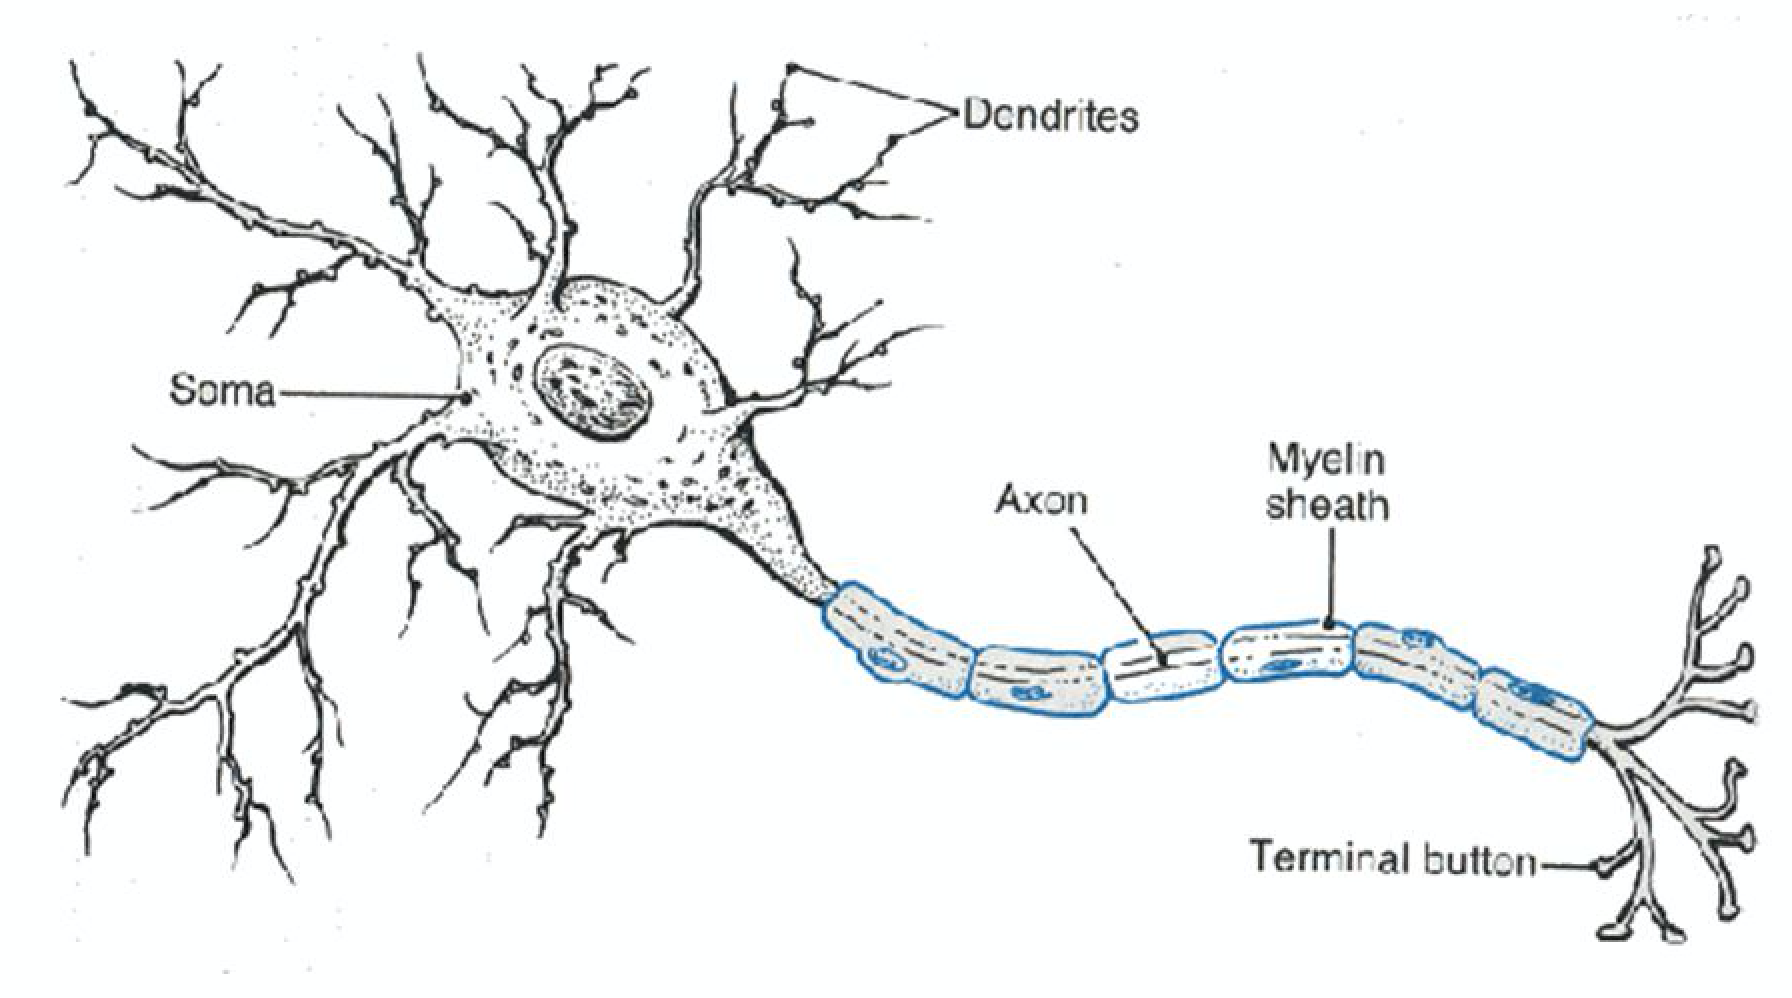
\includegraphics[height=3.5cm,width=\textwidth]{n1.png}
	\caption{Biological Neuron}
\end{subfigure}
\begin{subfigure}{0.5\linewidth}
	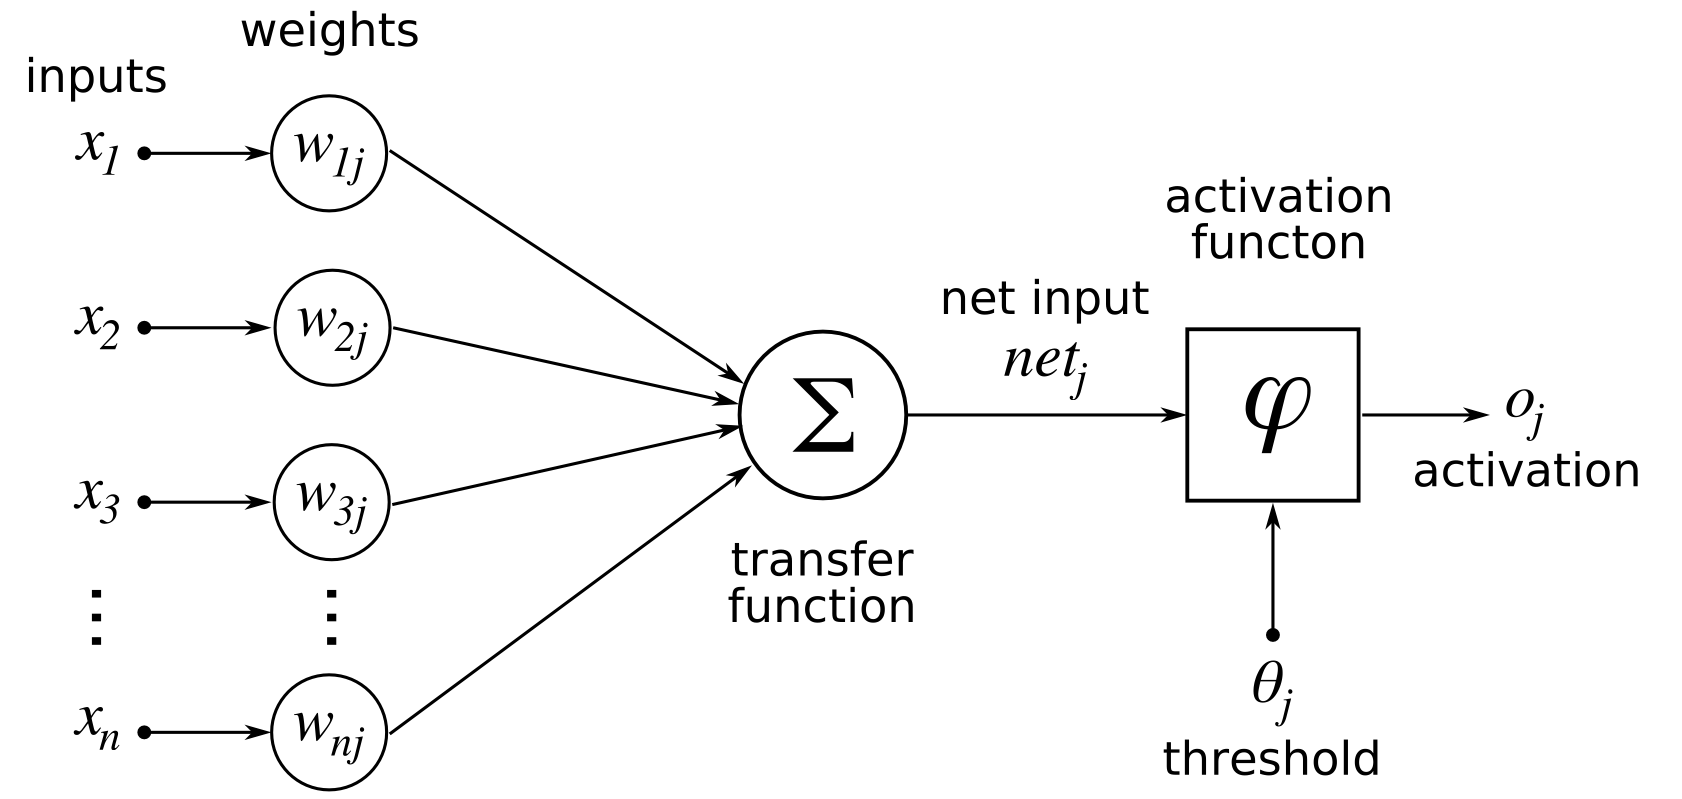
\includegraphics[height=3.5cm,width=\textwidth]{Aneuron.png}
	\caption{Artificial Neuron}
\end{subfigure}
\label{Biological Neuron and Artificial Neuron}
\caption{Biological Neuron and Artificial Neuron}
\end{figure}
An artificial neuron is an information cell which can compute input with some special algorithm and output results.An artificial neural network is composed of hundreds or thousands of neurons.Each neuron gets input from last layer neurons and output to next neurons.The first layer is called input layer, the last layer is output layer, and all layers between the input layer and output layer are the hidden layer.Normally, we consider the Artificial neural network as a black box. It read data in the input layer and output result after amounts of computation.\\

\begin{figure}[h]
\centering
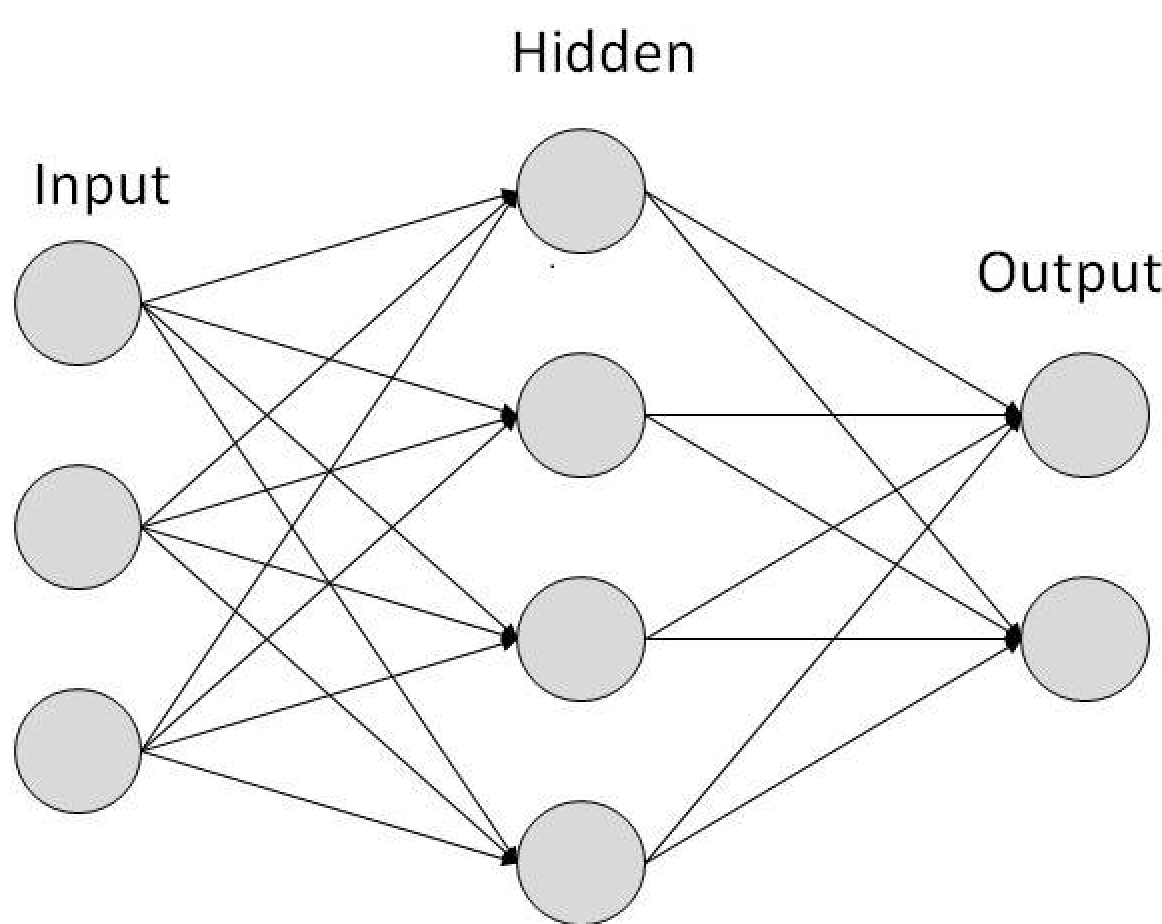
\includegraphics[height=3cm,width=0.4\textwidth]{nn1.png}
\caption{Neuron Network}
\end{figure}

\newpage

Like biological neurons have \textit{synapse}, each artificial neuron has a  computation cell called activation function. The activation function will decides whether and how much the data can output to next neuron.Next figure is showing different types activation function.Unlike biological neurons, artificial neurons also have weights and biases.Before input to activation function all inputs should go through a transfer function unit.\\

Transfer function:

\[z= \sum\limits_{i}W_i X_i +b\]

Activation function:
	\[\phi(z)\]
\begin{figure}[h]
\centering
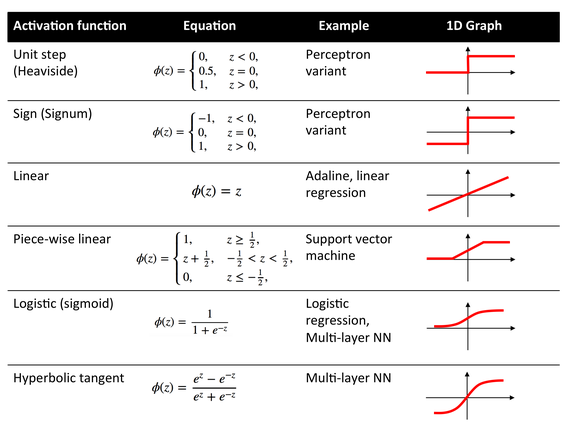
\includegraphics[width=0.9\textwidth]{activation.png}
\caption{Different types activation}
\end{figure}

\newpage

A neural network is not enough to do some real jobs, it only contains initialized parameters.To make it works, we need to train the neural network.Error backpropogation is a powerful weapen in almost all the real life jobs.A training iteration consists two parts, forward propagation and backward propagation(BP). As we mentioned, forward network pass  data from input layer until output layer, while backward pass error from output layer back to input layer.Before we dig deeper in BP, a loss function should be defined in advance. The loss function is a tool to evaluate  the difference (Error) between the output and the target output.In general, all the neural network jobs are always around the error.The goal is to minimize the error, to optimize the network parameters.A practical example is belowing to help understand Backpropagation and Gradient decent.

\textbf{Example for Backpropagation:}
Assume that every day you have lunch at the cafeteria, you diet only consists of fish , chips, and ketchup. The cashier only tells you the total price of the meal. A few days later, you should be able to figure out the single price of each food.

Assume price of means is 850, and use linear activation function and squared error function in this example.\\
Target Price: 850\\
Portions of fish: 2\\
Portions of chips: 5\\
Portions of ketchups:3\\
\[Price=X_{fish} W_{fish}+X_{chips}W_{chips}+X_{ketchup}W_{ketchup}\]
First we star with random guess the prices:
\[W_{fish}=W_{chips}=W_{ketchup}=50\]
$So,price=2\times 50+5\times 50+3\times 50=500$
\[E=\frac{1}{2} \sum\limits_{n\in training}(t^n-y^n)^2\]

\begin{figure}[h]
\centering
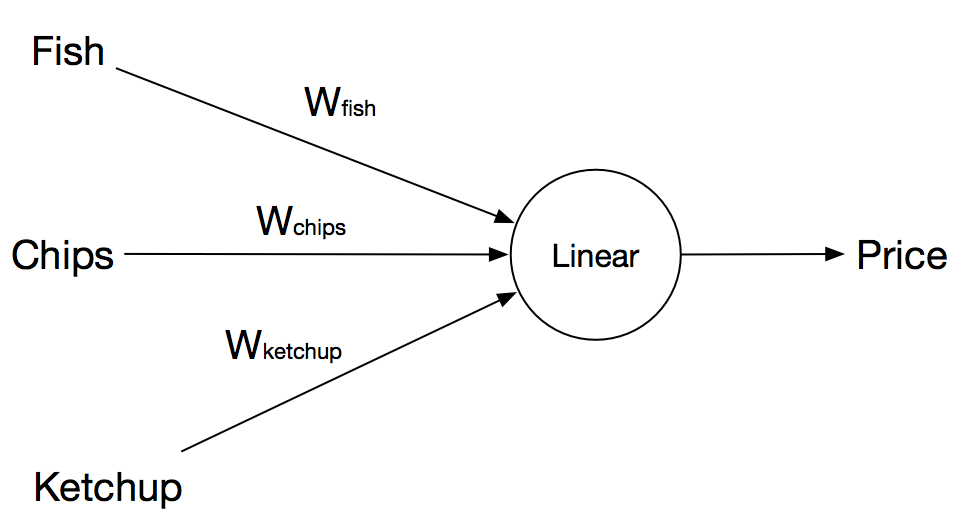
\includegraphics[width=0.5\textwidth]{bp.png}
\caption{BP example }
\end{figure}
\newpage
Where:
$t$ is target price,$y$ is output price, $\varepsilon$ is learning rate(assume 1/35).
\[\frac{\partial{E}}{\partial{w_i}}=\frac{1}{2}\sum\limits_n\frac{\partial{y^n}}{\partial{w_i}}\frac{d{E^n}}{d{y^n}} =-\sum\limits_n x_i^n(t^n-y^n)\]

\[\Delta w_i=-\varepsilon\frac{\partial E}{\partial w_i}=\sum\limits_n \varepsilon x_i^n(t^n-y^n)\]
In this case n=1.\\
Thus $ \Delta w_i =\frac{1}{35}x_i(850-500)$\\

$\Delta w_{fish}=20,\Delta w_{chips}=50,\Delta w_{ketchup}=30$   \\

Update to\\

$w_{fish}=70,w_{chips}=100,w_{ketchup}=80$  \\

$ Price=2\times 70+5\times 100+3\times 80=880$\\
 
One more iteration\\

$\Delta w_{fish}=-1.7,\Delta w_{chips}=-4.3,\Delta w_{ketchup}=-2.6$   \\

Update to\\

$w_{fish}=68.3,w_{chips}=95.7,w_{ketchup}=77.4$  \\

$price=2\times 68+5\times 95.7+3\times 77.4=847.3$\\
As the above computation  shows, total price is 500 , 880 then 847.3.With enough iterations, there is no doubt the total price will converge to 850, the target output.
\subsection{Convolution Neural Network(CNN)}
In image processing and computer vision field, the images are usually  represented as pixel vectors.For instance, there is a 1000 by 1000 image, so this image could be present as a 1000000-dimension vector.If the hidden layer has same number of neurons as input layer. Then the number of weights should equels 1000000*1000000=$10^{12}$. $10^{12}$ weight is too many to be trained.In other words, it is  impossible for hardware to process so many parameters.In order to process images in neural network, we have to reduce parameters.
\subsubsection{Local Connectivity}
In general, The spatial connection of the image is also the local pixel contact is more closely, and the distant pixel correlation is weak.Thus, each neuron is not necessary to perceive the global image, only need to perceive the local, and then at the higher level will be part of the information together to get the overall information.As the instance we mentioned before, assume each neuron only connects to 10*10 neurons, then paremeters will reduce from $10^{12}$ to $10^8$.In fact, it is equivalent to convolution operation.
\begin{figure}[h]
\centering
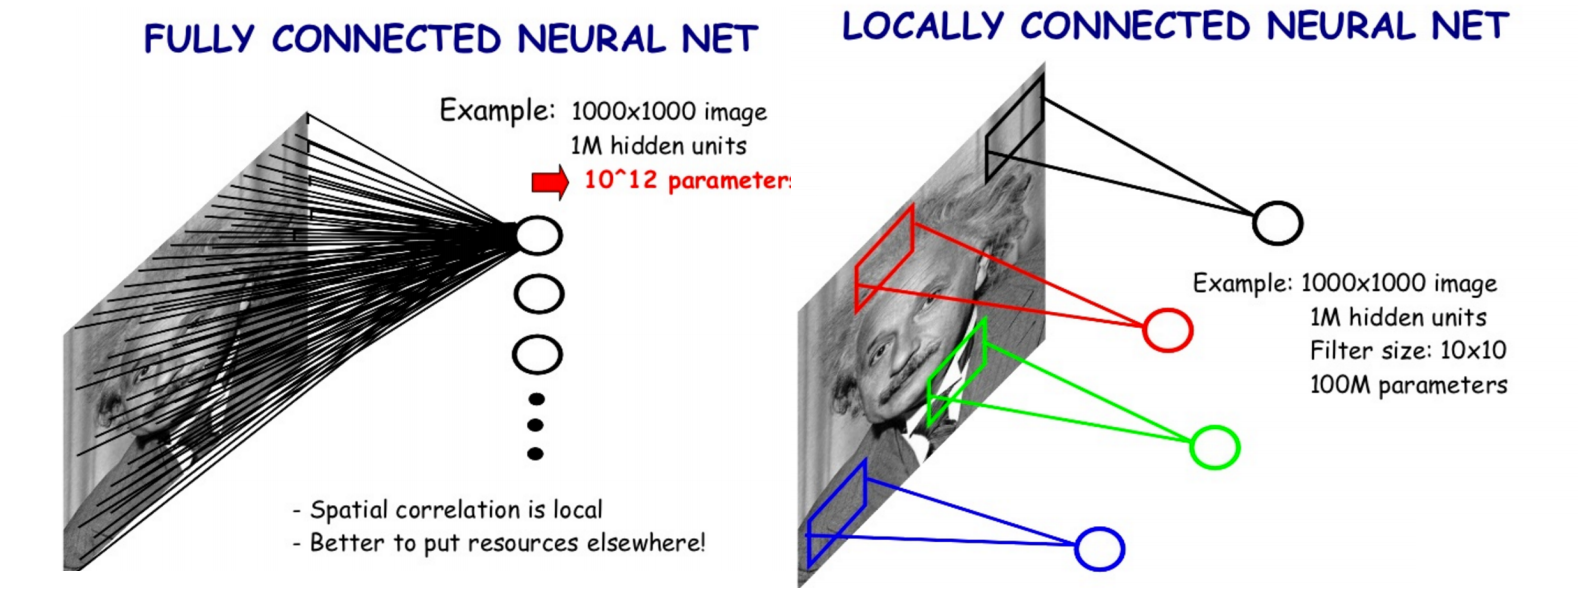
\includegraphics[width=0.9\textwidth]{localconnect.png}
\caption{Fully connected and local connected network}
\end{figure}
\subsubsection{Parameters Sharing}
However,$10^8$ parameters is still too large for a neural network.The other power weapon to reduce parameters is parameter sharing.In the above local connected instance, each neuron corresponds to 100 parameters, there are a total of 1000000 neurons.If  all the 1000000 neurons have the same 100 parameters, then the number of parameters reduce to 100.\\
\begin{figure}[h]
\centering
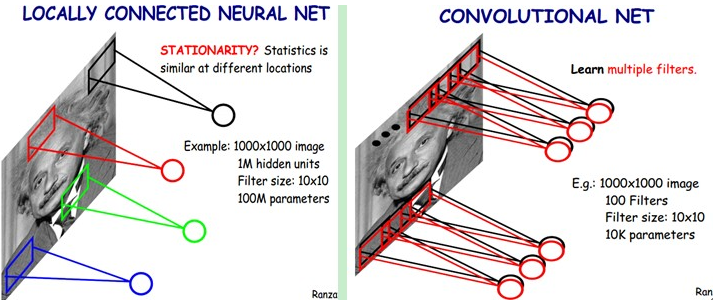
\includegraphics[height=4cm,width=0.9\textwidth]{parameter.png}
\caption{Multiple convolution kernels}
\end{figure}
To understand the weight of sharing better, we consider these 100 parameters (that is, convolution operations) as a way of extracting features that are independent of position. The implication of this is that the statistical properties of a part of the image are the same as those of the other parts. This also means that the features we learn in this part can also be used on another part, so we can use the same learning feature for all the positions on the image.Normally, one feature is not enough for an image, so it is better to use multiple kernel to learn multiple features.
\subsubsection{Convolution Layer}
convolution layer is the core layer of a convolutional neural network, which compute dot product between the filters and the input data. In image processing, input data usually has three dimension, width, height and depth. The convolution kernel depth has to match input volume	depth.In other words, the number of channels have to be same.	Next figure is showing a practical example of what convolution does.	
\begin{figure}[h]
\centering
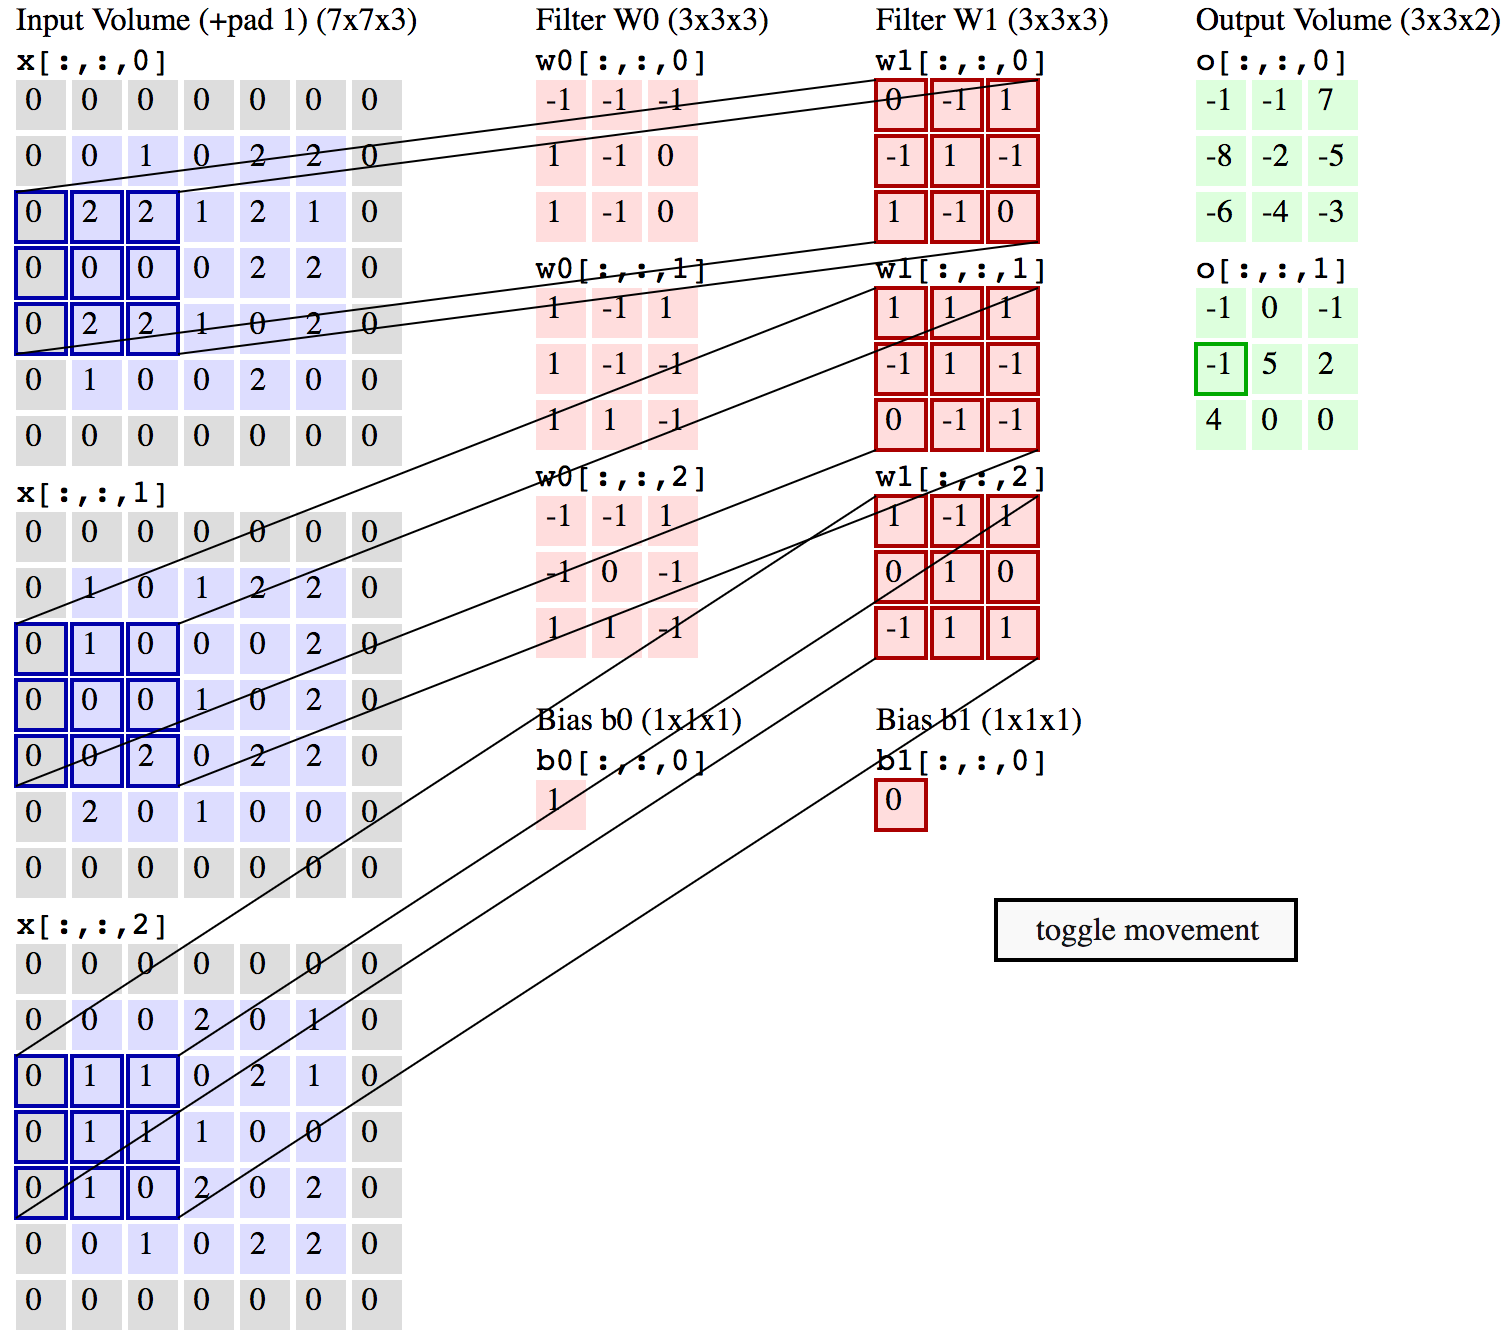
\includegraphics[width=0.9\textwidth]{conv.png}
\caption{Convolution}
\end{figure}

In general, if a convolution layer with:
\begin{itemize}
\item Input vulome with size $W_1\times H_1\times D_1$
\item Number of kernels K
\item Zero padding width P:the gray cell with value 0 in fugure 5, zero padding is only for controling of output shape.
\item The stride S:step size of sliding kernel.
\item Kernel size F
\end{itemize}

Produce a volume of size $W_2 \times H_2 \times D_2$ where:
\begin{itemize}
\item $W_2=(W_1-F+2P)/S+1$
\item $H_2=(H_1-F+2P)/S+1$
\item $D_2=K$
\end{itemize}

The input volume size is 5x5x3,zero padding size 2, with two 3x3x3 kernels.
\begin{itemize}
\item $W_2=(5-3+2 \times 1)/2+1=3$
\item $H_2=(5-3+2 \times 1)/2+1=3$
\item $D_2=2$
\end{itemize}
With the equation we can easily compute output volume shape 3x3x2.

\newpage
\subsubsection{Pooling Layer}
After convolution layer, the next step is to use these features to do the classification jobs. Theoretically, we can use all the extracted features to train the classifier, such as the softmax classifier, but this is facing with the challenge of calculating the amounts of computation and overfitting.A pooling layer is usually followed a convolution layer to control overfitting and spatial size of data.The most common form is a pooling layer with 2x2 size kernels which match the depth to input volume.At most of time, the kernel with a stride of 2.Assume a Max poling is applied, that means the operation will pick the maximum value from every possible  2x2 region.

\begin{figure}[h]
\centering
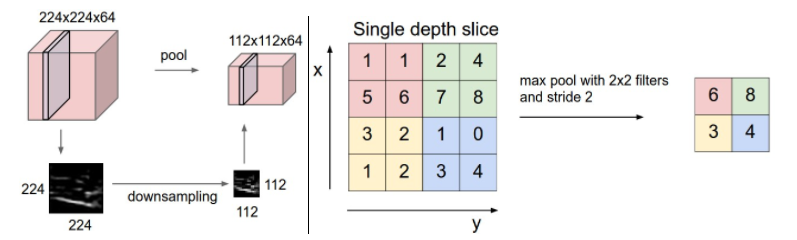
\includegraphics[width=0.9\textwidth]{pooling.png}
\caption{Pooling operation}
\end{figure}
In summary, a pooling layer with:
\begin{itemize} 
\item input volume $W_1 \times H_1 \times D_1$
\item filter size F
\item stride S

Produces an output volume$W_2 \times H_2 \times D_2$, where:
\item $W_2=(W_1-F)/S+1$
\item $H_2=(H_1-F)/S+1$
\item $D_2=D_1$
\end{itemize}

\newpage

\subsubsection{Some Popular CNN Architectures}
\begin{itemize}
\item \textbf{LeNet:} First successful CNN Architecture which developed by Yann LeCun in 90s.
\begin{figure}[h]
\centering
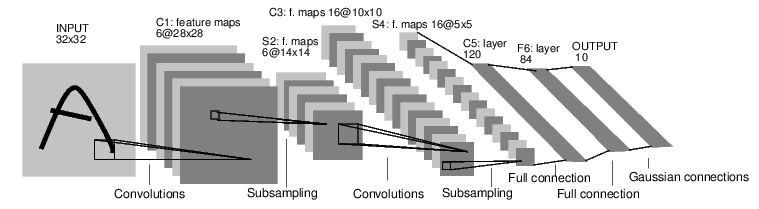
\includegraphics[width=0.8\textwidth]{lenet.png}
\caption{LeNet Architecture}
\end{figure}
\item \textbf{AlexNet:} AlexNet was developed by Alex Krizhevsky, Ilya Sutskever and Geoff Hinton. The AlexNet achieved second runner-up in ImageNet ILSVRC challenge in 2012.It was  very similar to LeNet, but bigger and deeper than it.
\begin{figure}[h]
\centering
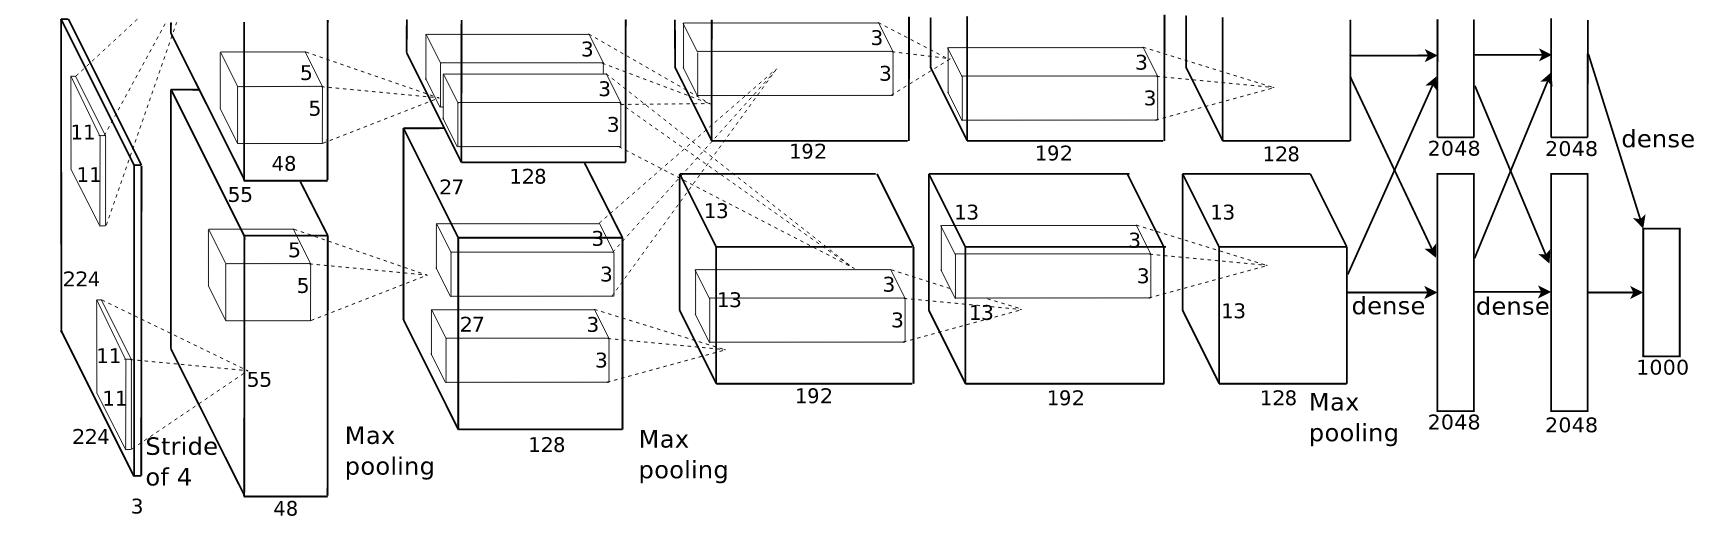
\includegraphics[width=0.8\textwidth]{alexnet.png}
\caption{AlexNet Architecture}
\end{figure}
\item \textbf{ZFNet:} ZFNet was a provement version of AlexNet which came from Matthew Zeiler and Rob Fergus.The CNN architecture also made  them winner in ILSVRC 2013.Compare to AlexNet, ZFNet has bigger size of middle convolution kernel and smaller stride.
\item \textbf{GoogleNet:}  Szegedy et al was the author of GooleNet, and he also won the ILSVRC 2014.GoogleNet reduce a large amount of  parameters from 60M to 4M(compared to AlexNet).
\item \textbf{VGGNet:}VGGNet was runner-up in ILSVRC 2014 which came from Karen Simonyan and Andrew Zisserman.The VGGNet proved that deeper neural network not always have better perfermance.On the other side VGGNet cost a lot of memory for parameters(14M).In this project we use VGG-16 which composed of 13 convolution layers and 3  fully connected layers.

\begin{figure}[h]
\centering
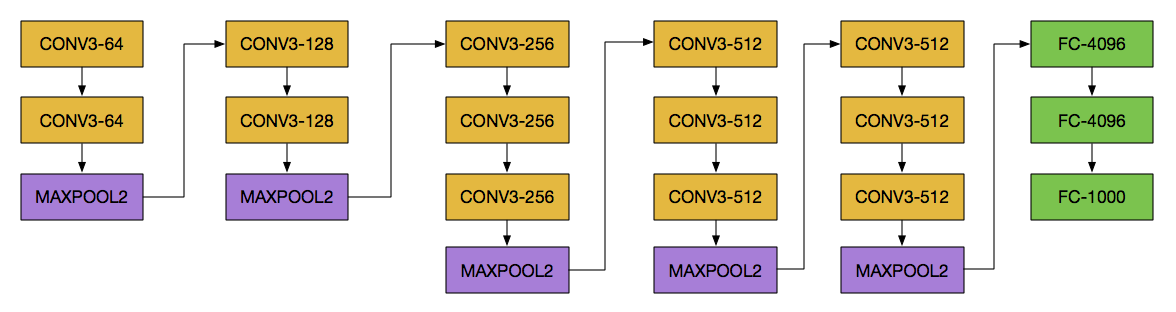
\includegraphics[width=0.9\textwidth]{vgg16.png}
\caption{VGG-16 Architecture}
\end{figure}

\end{itemize}
\newpage
\section{Requirements Specification}
\section{Design}
\section{Implementation and Testing}
\section{Evaluation}
\section{Appraisal}
\section{Summary and Conclusion}
\section{Recommendation for Future Work}
\end{document}